\documentclass[tikz,border=0pt]{standalone}
\usepackage{xcolor}
% Palette: Sam_Comm_final.png by eye, and the woods' own colours.
\definecolor{ink}{HTML}{3B2340}
\definecolor{sky}{HTML}{EFC46A}
\definecolor{skyhi}{HTML}{F5DA92}
\definecolor{skylow}{HTML}{E9B060}
\definecolor{cloud}{HTML}{F2D58A}
\definecolor{dusk}{HTML}{E99A6A}
\definecolor{duskhi}{HTML}{F0B07E}
\definecolor{dusklow}{HTML}{C9746A}
\definecolor{coral}{HTML}{E88A73}
\definecolor{salmon}{HTML}{EE9F7E}
\definecolor{rose}{HTML}{E47A7E}
\definecolor{peach}{HTML}{F0B07E}
\definecolor{grass}{HTML}{8DBB7E}
\definecolor{grassdark}{HTML}{6FA77A}
\definecolor{grasslight}{HTML}{A9C97F}
\definecolor{pine}{HTML}{5E9C6A}
\definecolor{teal}{HTML}{4FA3A5}
\definecolor{farpine}{HTML}{B7C98A}
\definecolor{hill}{HTML}{C9C078}
\definecolor{hillfar}{HTML}{E3C483}
\definecolor{clearing}{HTML}{B9CF86}
\definecolor{dirt}{HTML}{D3A77D}
\definecolor{dirtdark}{HTML}{B98A64}
\definecolor{stone}{HTML}{A8B0A4}
\definecolor{trunk}{HTML}{B9835A}
\definecolor{trunkdark}{HTML}{8C5A44}
\definecolor{mushroom}{HTML}{F26B38}
\definecolor{silk}{HTML}{F6E7C4}
\definecolor{flower}{HTML}{FF6F91}
\definecolor{flowergold}{HTML}{FFB000}
\definecolor{leafgold}{HTML}{F2B53A}
\definecolor{mud}{HTML}{B9835A}
\definecolor{muddark}{HTML}{8C5A44}
\definecolor{cream}{HTML}{EBC592}
\definecolor{blush}{HTML}{F08A8A}
\definecolor{bone}{HTML}{FBF4E4}
\definecolor{crabshell}{HTML}{D2463C}
\definecolor{crabdark}{HTML}{A8323A}
\definecolor{wing}{HTML}{CDE8E0}
\definecolor{goldbelt}{HTML}{F2B53A}
\definecolor{stag}{HTML}{A8693C}
\definecolor{stagdark}{HTML}{7E4A2C}
\definecolor{antler}{HTML}{E2C79A}
\definecolor{moss}{HTML}{6FA77A}
\definecolor{eyeglow}{HTML}{FFE38A}
\definecolor{chitin}{HTML}{6B4E71}
\definecolor{chitinhi}{HTML}{8E6E94}
\definecolor{acorn}{HTML}{C98A55}
\definecolor{acorncap}{HTML}{8C5A44}
\definecolor{fire}{HTML}{FF8A3D}
\definecolor{firehi}{HTML}{FFE38A}
\definecolor{jar}{HTML}{CDE8E0}
\definecolor{white}{HTML}{FFFFFF}
\begin{document}
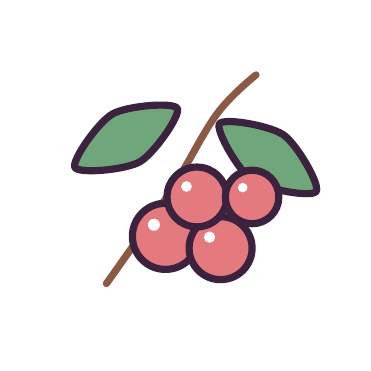
\begin{tikzpicture}
\clip (0,0) rectangle (4,4);
\draw[trunkdark, line width=2.6pt, line cap=round, line join=round] plot[smooth, tension=0.6] coordinates {(1,0.75) (1.8,1.9) (2.4,2.9) (2.9,3.4)};
\filldraw[draw=ink, line width=2.6pt, line join=round, fill=grassdark] plot[smooth cycle, tension=0.5] coordinates {(0.6,2.225) (1.075,2.903) (1.9,2.975) (1.425,2.297)};
\filldraw[draw=ink, line width=2.6pt, line join=round, fill=grassdark] plot[smooth cycle, tension=0.5] coordinates {(2.436,2.78) (3.251,2.637) (3.664,1.92) (2.849,2.063)};
\filldraw[draw=ink, line width=2.6pt, line join=round, fill=rose] (1.75,1.35) circle (0.42);
\fill[white] (1.603,1.497) circle (0.076);
\filldraw[draw=ink, line width=2.6pt, line join=round, fill=rose] (2.45,1.2) circle (0.4);
\fill[white] (2.31,1.34) circle (0.072);
\filldraw[draw=ink, line width=2.6pt, line join=round, fill=rose] (2.15,1.85) circle (0.38);
\fill[white] (2.017,1.983) circle (0.068);
\filldraw[draw=ink, line width=2.6pt, line join=round, fill=rose] (2.85,1.85) circle (0.34);
\fill[white] (2.731,1.969) circle (0.061);
\end{tikzpicture}
\end{document}
